% Options for packages loaded elsewhere
\PassOptionsToPackage{unicode}{hyperref}
\PassOptionsToPackage{hyphens}{url}
%
\documentclass[
  man]{apa7}
\usepackage{amsmath,amssymb}
\usepackage{iftex}
\ifPDFTeX
  \usepackage[T1]{fontenc}
  \usepackage[utf8]{inputenc}
  \usepackage{textcomp} % provide euro and other symbols
\else % if luatex or xetex
  \usepackage{unicode-math} % this also loads fontspec
  \defaultfontfeatures{Scale=MatchLowercase}
  \defaultfontfeatures[\rmfamily]{Ligatures=TeX,Scale=1}
\fi
\usepackage{lmodern}
\ifPDFTeX\else
  % xetex/luatex font selection
\fi
% Use upquote if available, for straight quotes in verbatim environments
\IfFileExists{upquote.sty}{\usepackage{upquote}}{}
\IfFileExists{microtype.sty}{% use microtype if available
  \usepackage[]{microtype}
  \UseMicrotypeSet[protrusion]{basicmath} % disable protrusion for tt fonts
}{}
\makeatletter
\@ifundefined{KOMAClassName}{% if non-KOMA class
  \IfFileExists{parskip.sty}{%
    \usepackage{parskip}
  }{% else
    \setlength{\parindent}{0pt}
    \setlength{\parskip}{6pt plus 2pt minus 1pt}}
}{% if KOMA class
  \KOMAoptions{parskip=half}}
\makeatother
\usepackage{xcolor}
\usepackage{graphicx}
\makeatletter
\def\maxwidth{\ifdim\Gin@nat@width>\linewidth\linewidth\else\Gin@nat@width\fi}
\def\maxheight{\ifdim\Gin@nat@height>\textheight\textheight\else\Gin@nat@height\fi}
\makeatother
% Scale images if necessary, so that they will not overflow the page
% margins by default, and it is still possible to overwrite the defaults
% using explicit options in \includegraphics[width, height, ...]{}
\setkeys{Gin}{width=\maxwidth,height=\maxheight,keepaspectratio}
% Set default figure placement to htbp
\makeatletter
\def\fps@figure{htbp}
\makeatother
\setlength{\emergencystretch}{3em} % prevent overfull lines
\providecommand{\tightlist}{%
  \setlength{\itemsep}{0pt}\setlength{\parskip}{0pt}}
\setcounter{secnumdepth}{-\maxdimen} % remove section numbering
% Make \paragraph and \subparagraph free-standing
\ifx\paragraph\undefined\else
  \let\oldparagraph\paragraph
  \renewcommand{\paragraph}[1]{\oldparagraph{#1}\mbox{}}
\fi
\ifx\subparagraph\undefined\else
  \let\oldsubparagraph\subparagraph
  \renewcommand{\subparagraph}[1]{\oldsubparagraph{#1}\mbox{}}
\fi
\ifLuaTeX
\usepackage[bidi=basic]{babel}
\else
\usepackage[bidi=default]{babel}
\fi
\babelprovide[main,import]{english}
% get rid of language-specific shorthands (see #6817):
\let\LanguageShortHands\languageshorthands
\def\languageshorthands#1{}
% Manuscript styling
\usepackage{upgreek}
\captionsetup{font=singlespacing,justification=justified}

% Table formatting
\usepackage{longtable}
\usepackage{lscape}
% \usepackage[counterclockwise]{rotating}   % Landscape page setup for large tables
\usepackage{multirow}		% Table styling
\usepackage{tabularx}		% Control Column width
\usepackage[flushleft]{threeparttable}	% Allows for three part tables with a specified notes section
\usepackage{threeparttablex}            % Lets threeparttable work with longtable

% Create new environments so endfloat can handle them
% \newenvironment{ltable}
%   {\begin{landscape}\centering\begin{threeparttable}}
%   {\end{threeparttable}\end{landscape}}
\newenvironment{lltable}{\begin{landscape}\centering\begin{ThreePartTable}}{\end{ThreePartTable}\end{landscape}}

% Enables adjusting longtable caption width to table width
% Solution found at http://golatex.de/longtable-mit-caption-so-breit-wie-die-tabelle-t15767.html
\makeatletter
\newcommand\LastLTentrywidth{1em}
\newlength\longtablewidth
\setlength{\longtablewidth}{1in}
\newcommand{\getlongtablewidth}{\begingroup \ifcsname LT@\roman{LT@tables}\endcsname \global\longtablewidth=0pt \renewcommand{\LT@entry}[2]{\global\advance\longtablewidth by ##2\relax\gdef\LastLTentrywidth{##2}}\@nameuse{LT@\roman{LT@tables}} \fi \endgroup}

% \setlength{\parindent}{0.5in}
% \setlength{\parskip}{0pt plus 0pt minus 0pt}

% Overwrite redefinition of paragraph and subparagraph by the default LaTeX template
% See https://github.com/crsh/papaja/issues/292
\makeatletter
\renewcommand{\paragraph}{\@startsection{paragraph}{4}{\parindent}%
  {0\baselineskip \@plus 0.2ex \@minus 0.2ex}%
  {-1em}%
  {\normalfont\normalsize\bfseries\itshape\typesectitle}}

\renewcommand{\subparagraph}[1]{\@startsection{subparagraph}{5}{1em}%
  {0\baselineskip \@plus 0.2ex \@minus 0.2ex}%
  {-\z@\relax}%
  {\normalfont\normalsize\itshape\hspace{\parindent}{#1}\textit{\addperi}}{\relax}}
\makeatother

\makeatletter
\usepackage{etoolbox}
\patchcmd{\maketitle}
  {\section{\normalfont\normalsize\abstractname}}
  {\section*{\normalfont\normalsize\abstractname}}
  {}{\typeout{Failed to patch abstract.}}
\patchcmd{\maketitle}
  {\section{\protect\normalfont{\@title}}}
  {\section*{\protect\normalfont{\@title}}}
  {}{\typeout{Failed to patch title.}}
\makeatother

\usepackage{xpatch}
\makeatletter
\xapptocmd\appendix
  {\xapptocmd\section
    {\addcontentsline{toc}{section}{\appendixname\ifoneappendix\else~\theappendix\fi\\: #1}}
    {}{\InnerPatchFailed}%
  }
{}{\PatchFailed}
\DeclareDelayedFloatFlavor{ThreePartTable}{table}
\DeclareDelayedFloatFlavor{lltable}{table}
\DeclareDelayedFloatFlavor*{longtable}{table}
\makeatletter
\renewcommand{\efloat@iwrite}[1]{\immediate\expandafter\protected@write\csname efloat@post#1\endcsname{}}
\makeatother
\usepackage{lineno}

\linenumbers
\usepackage{csquotes}
\makeatletter
\renewcommand{\paragraph}{\@startsection{paragraph}{4}{\parindent}%
  {0\baselineskip \@plus 0.2ex \@minus 0.2ex}%
  {-1em}%
  {\normalfont\normalsize\bfseries\typesectitle}}

\renewcommand{\subparagraph}[1]{\@startsection{subparagraph}{5}{1em}%
  {0\baselineskip \@plus 0.2ex \@minus 0.2ex}%
  {-\z@\relax}%
  {\normalfont\normalsize\bfseries\itshape\hspace{\parindent}{#1}\textit{\addperi}}{\relax}}
\makeatother

\ifLuaTeX
  \usepackage{selnolig}  % disable illegal ligatures
\fi
\IfFileExists{bookmark.sty}{\usepackage{bookmark}}{\usepackage{hyperref}}
\IfFileExists{xurl.sty}{\usepackage{xurl}}{} % add URL line breaks if available
\urlstyle{same}
\hypersetup{
  pdftitle={Introduction},
  pdfauthor={Jimmy},
  pdflang={en-EN},
  hidelinks,
  pdfcreator={LaTeX via pandoc}}

\title{Introduction}
\author{Jimmy\textsuperscript{}}
\date{}


\shorttitle{SHORT TITLE}

\affiliation{\phantom{0}}

\begin{document}
\maketitle

Moderation analysis plays an important role in social science research because it can illuminate the intricate nature of human behaviors and allows for differential effects among explanatory variables. Social scientists use the terms ``moderation'' and ``interaction'' interchangeably since both refer to how a third variable can modify the relation between two variables (Fairchild \& McQuillin, 2010). Baron and Kenny's (1986) groundbreaking work on moderation emphasized the need to understand not only the existence of an effect but also the circumstances that shaped it. Alternatively speaking, interaction effects reveal how the strength and direction of relations between variables can shift depending on contextual factors. For instance, it was found that the number of passive and active bystanders in a work group moderated the relationship between exposure to bullying and work engagement (Ng et al., 2022). Typical interaction effects are frequently investigated through regression-based techniques (Hayes \& Rockwood, 2017; Hayes, 2013), in which an interaction term is created by multiplying the explanatory variable with the interacting variable and then included in the regression model.

A significant limitation of traditional regression-based approaches with observed variables is that directly measured variables are inherently subject to measurement error. This practice usually results in reduced statistical power and has the potential to obscure true relationships, and thus fails to detect nuanced interaction effects (Busemeyer \& Jones, 1993; Atkinson \& Nevill, 1998; Yezerinac et al., 1992; Fritz, Kenny, \& MacKinnon , 2016). To address these potential concerns, researchers may consider latent variables to account for measurement error. Latent variables are not directly observable but inferred from observed indicators or manifest variables (Bollen 1989), such as anxiety measured by Beck Anxiety Inventory (BAI; Beck et al., 1993). To model relations between latent variables, researchers extensively use structural equation modeling (SEM) in which a network of equations not only captures relations between observed indicators and their underlying latent variables but also models the relationships among the latent variables themselves (Bollen, 1989; Hoyle, 1995).This simultaneous modeling of measurement model and structural paths enables a comprehensive assessment of complex theoretical models, providing insights into mediation and moderation within a single analysis (Kline, 2015). Hence, typical regression models with interaction can be tested among latent variables.

Since the relations between latent variables can only be investigated through observed indicators, it is not possible to directly multiply them as observed variables. In past years, a few latent interaction models have been developed based on the SEM framework (Jaccard \& Wan, 1995; Jöreskog \& Yang, 1996; Ping, 1998; Klein \& Moosbrugger, 2000; Wall \& Amemiya, 2001; Marsh et al., 2004; Maslowsky et al., 2014; Hsiao et al., 2018). These methods can be divided into two categories: product indicator methods and distribution analytic methods (Marsh et al., 2012). Latent moderated structural equations (LMS) is a widely used method based on the distribution analytic method, but it is limited in use since it does not generate model fit indices and standard coefficients for interaction effects, hence making model comparisons and coefficient interpretations difficult (Malowsky et al., 2014). Therefore we focus on product indicator methods in this study.

The present paper used a nationally representative dataset to demonstrate the application of three product indicator methods of estimating latent interaction effects and compare the results in terms of parameter estimates and implementing procedure: unconstrained product indicator (UPI; Marsh et al., {[}2004{]}), reliability-adjusted product indicator (RAPI; Hsiao et al., {[}2018{]}), and two-stage path analysis with interaction (2S-PA-Int; Lai \& Hsiao, {[}2021{]}). The performance of each method has been evaluated through simulation studies in each stemming paper, but only UPI is commonly used in empirical studies of latent interaction and demonstrated with concrete examples. This paper aims to: (1) provide detailed demonstration of each method on an existing dataset with an empirically supported theory; (2) supplement the comparison of three product indicator methods in simulated settings; (3) examine the moderating effect of self-esteem on the relations between perceived everyday discrimination on depression using latent variable modeling. In the demonstration, we expect to detect a significant latent interaction effect using all the methods.

\hypertarget{perceived-everyday-discimination-self-esteem-and-depression}{%
\subsection{Perceived Everyday Discimination, Self-Esteem, and Depression}\label{perceived-everyday-discimination-self-esteem-and-depression}}

Emerging adulthood, defined as ages of 18 to mid-to-late 20s, has been gaining attention in cognitive, social, and clinical psychology research. It is recognized as a pivotal developmental stage typified by what they pursue, how they strive, and where they will be (Arnett, 2000). This is a stimulating yet stressful period filled with relatively more changes and challenges in an individual's lifespan, given that people in this transition period (i.e., childhood to young adulthood) usually need to make major life decisions, take responsibility for their own needs, and explore their future (Wagner \& Newman, 2012). Numerous research reported that emerging adulthood is typically connected to the onset of various mental health illnesses and the development of serious mental health conditions that exacerbate later health (Klodnick et al., 2021). Specifically, emerging adults are more prone to depressive symptoms that lead to suicidal tendencies, feeling of worthlessness, sleeping trouble, and social avoidence (Martínez-Hernáez et al., 2016).
Many potential stress factors may culminate in the depressive symptoms described above, given the abundance of challenges young adults may have to confront in their everyday social interaction. Current social and clinical research have found that perceived everyday discrimination (PED) is significantly associated with depression among emerging adults in the United States (\textbf{williamsRacialEthnicDiscrimination2003?}). PED is defined as ``a behavioral manifestation of a negative attitude, judgment, or unfair treatment toward members of a group'' through subjective evaluations (\textbf{pascoePerceivedDiscriminationHealth2009a?}). For instance, LGBT individuals perceive significantly higher levels of sexual-orientation-related discrimination, which results in greater likelihood of incurring depression, compared to their heterosexual counterparts (\textbf{burgessEffectsPerceivedDiscrimination2007?}). Living in an immigrant country brimming with people from different cultural backgrounds, racial minorities may encounter discrimination related to their race and ethnicity in various settings. (\textbf{patrickEffectRacialDiscrimination2019?}) found that PED and experience of related violence may lead to increased depression among African American and Hispanic American adolescents.

Self-esteem has been researched as one of the correlates that potentially alleviate the effect of PED on depression. In Rosenberg's work, self-esteem is early characterized as ``a favorable or unfavorable attitude toward oneself and functions as an affective evaluation of the self'' (Rosenberg, 1965). A more recent definition is that self-esteem depicts a psychological approximation of the degree to which one individual is evaluated and accepted by themselves and others (e.g., peers, family, friends; Harter, 2003). Individuals with high self-esteem have higher chances of perceiving subjective well-being and obtaining self-confidence in adolescents and adults (Weinberg \& Gould, 1995; Chen et al., 2016). From an intuitive perspective, individuals with low or reduced level of self-esteem are more plausible to possess lower self-assurance and experience more detrimental emotional consequences resulting from PED. One study about second-generation immigrant adolescents across ethnic groups confirmed this pathway, in which PED from school peers negatively influences perceptions of social acceptance and subsequently impacts their mental health outcomes (Espinosa, 2021). Moreover, it was found that gender-related PED predicts increased psychological malfunctioning through both linear and non-linear reduction in self-esteem among American Indians. (Kira et al., 2015).

Although the moderation effect of self-esteem on mental health outcomes has been studied in various representative samples across groups and occasions (Chen et al., 2022; Hart et al., 2022), few studies model this effect in a latent variable framework. The current study posits self-esteem as a moderator of the relation between PED and depression among emerging adults (18-28) in the United States. The hypotheses are three-folds: (1) self-esteem is negatively associated with depression; (2) PED is positively associated with depression; (3) emerging adults who have higher levels of self-esteem will be less affected by PED on depression.

\hypertarget{three-product-indicator-methods-for-testing-latent-interaction}{%
\subsection{Three Product Indicator Methods for Testing Latent Interaction}\label{three-product-indicator-methods-for-testing-latent-interaction}}

Kenny and Judd's (1984) seminal idea on latent interaction has become the basis of many advanced approaches, especially for product indicators methods. They first proposed that the latent interaction term could be measured by all possible cross products of first-order indicators (i.e., observed indicators of latent predictors that formed the interaction term), and these products can form the product indicators (PIs) that indicate the latent interaction term. For example, suppose a latent predictor \(\xi_{x}\) and a latent moderator \(\xi_{m}\) are indicated by three first-order indicators respectively (i.e., \(\xi_{x}\) indicated by \(x_{1}\) \textasciitilde{} \(x_{3}\); \(\xi_{m}\) indicated by \(m_{1}\) \textasciitilde{} \(m_{3}\)), the formed PIs will be 9 PIs: \(x_{1}m_{1}\), \(x_{1}m_{2}\), \(x_{1}m_{3}\), \(x_{2}m_{1}\), \ldots, \(x_{3}m_{3}\). It can be observed that these PIs have shared first-order indicators, and hence their error variances covary (e.g., \(x_{1}m_{1}\) and \(x_{1}m_{2}\) share partial variances stemming from \(x_{1}\)). The Kenny and Judd's model is usually called constrained product indicator (CPI) method because it requires complicated nonlinear constraints on PIs (e.g., factor loadings and residual variances) in their model, which makes it difficult to implement and computationally burdensome for empirical researchers (Jaccard \& Wan, 1995). Take the PI \(x_{2}m_{2}\) as one example:
\begin{equation}
x_{2}m_{2}= (\lambda_{x_{2}}\xi_{x} + \delta_{x_{2}})(\lambda_{m_{2}}\xi_{m} + \delta_{m_{2}}),
\end{equation}
where \(\lambda\) is the factor loading, \(\xi\) is the first-order latent variable, and \(\delta\) is the error for first-order indicators \(x_{1}\) and \(m_{1}\). By expanding the equation, \(\lambda_{x_{2}m_{2}} = \lambda_{x_{2}}\lambda_{m_{2}}\), indicating that the factor loading of this PI is composed of original first-order indicators' factor loadings. The error variance can be derived as a function of original first-order indicators' error variances and first-order latent variables' variances. As the number of PIs increases, the complexity of nonlinear constraints is extremely challenging for model specification and may lead to convergence issue (Wall \& Amemiya, 2001). Moreover, this method is based on the assumption that first-order latent variables are normally distributed, which menas that CPI may not perform well when this assumption is violated. Marsh et al.~(2004) showed that CPI was not robust to non-normal data in their simulation studies, supporting the theoretical hypothesis.

\hypertarget{matched-pair-unconstrained-product-indicator-upi}{%
\subsubsection{Matched-pair Unconstrained Product Indicator (UPI)}\label{matched-pair-unconstrained-product-indicator-upi}}

As CPI is too complicated for researchers who do not have sufficient background in statistical details of SEM, Marsh et al.~(2004) proposed a groundbreaking method, unconstrained product indicator (UPI), to explore the possibility of removing complicated nonlinear constraints. UPI uses mean-centered first-order indicators to form PIs that indicate the latent interaction term, and omits most of the nonlinear constraints but the mean structure of latent variables, such that \(\kappa = [0, \ 0, \ Cov_{\xi_{x}\xi_{m}}]^T\) where \(\kappa\) represents a vector of latent means. Using the example mentioned before, the means of \(\xi_{x}\) and \(\xi_{m}\) are fixed to 0 and the mean of the interaction effect, \(Cov_{\xi_{x}\xi_{m}}\), equals the covariance between \(\xi_{x}\) and \(\xi_{m}\). It is necessary to keep the \(\kappa\) because \(Cov_{\xi_{x}\xi_{m}} \neq 0\) when \(\xi_{x}\) and \(\xi_{m}\) are allowed to correlate, so that the mean of the interaction term should be freely estimated. Marsh et al.~(2004) found that UPI without nonlinear constraints produced unbiased estimates of interaction effects and showed better performance under the violation of assumptions on normal distribution. They also argued that UPI could be more easily implemented than CPI, and therefore testing latent interaction should become more approachable and motivating when empirical researchers need to test more in-depth theories.

Although UPI with all PIs seems as a promising approach to use, it may lead to unrealistic model specification and risk of non-convergence when the number of PIs is overwhelmingly large. Marsh et al.~(2004) suggests to use matched-pair UPI by pairing up first-order indicators of two latent predictors in the order of reliability. For example, the formed PIs will be \(x_{1}m_{1}\), \(x_{2}m_{2}\) and \(x_{3}m_{3}\) instead of all the 9 possible configurations, assuming the order of indicators is by their reliability. Since nonlinear constraints are omitted, the factor loadings and error variances of formed PIs are freely estimated. Thus, we demonstrated matched-pair UPI in this study because Marsh et al.~(2004) showed that it was more favorable in terms of parsimonious model and comparably good performance.

\hypertarget{reliability-adjusted-product-indicator-rapi}{%
\subsubsection{Reliability-Adjusted Product Indicator (RAPI)}\label{reliability-adjusted-product-indicator-rapi}}

To further simplify the model, Marsh et al.~(2004) did propose a single indicator (SI) approach by using only one PI formed by first indicators of respective latent variables; however, nonlinear constraints should be applied again to the model for the identification issue (see pp.~279 in Marsh et al.~{[}2004{]}). They concluded that this method failed to show desirable performance because it disregarded most of available information from other unused first-order indicators. As a better alternative, a reliability-adjustment product indicator (RAPI) method using composite scores (sum or mean scores) was introduced in Hsiao et al.~(2018). The use of composite scores addresses the issue of unused information because composite scores could sufficiently and effectively gather all available information by using composite scores as SIs. More importantly, the RAPI model maintains simplicity. Using the reliability estimates of first-order indicators, RAPI places error-variance constraints on observed SIs to account for measurement error. Hsiao et al.~(2021) showed that RAPI exhibited the capability of generating unbiased estimates of latent interaction effects with acceptable standard errors under the condition of small sample size (\(\textit{N}\) = 250) and low reliability (\(\mathit{\rho}\) = .70) on congeneric items (i.e., items with differential factor loadings and measurement errors). Thus RAPI should be a good representative of SI approach for estimating latent interaction effects, and it was included in our demonstration.

\hypertarget{two-stage-path-analysis-with-interaction-2s-pa-int}{%
\subsection{Two-stage Path Analysis with Interaction (2S-PA-Int)}\label{two-stage-path-analysis-with-interaction-2s-pa-int}}

The Two-Stage Path Analysis (2S-PA) technique is an advanced method for modeling latent variables within the SEM framework, which has been shown to yield parameter estimates with reduced bias in standard errors, improved convergence rates, and less Type I error, particularly in smaller samples (Lai \& Hsiao, 2021). Similar to RAPI, 2S-PA is a SI approach when first-order indicators are continuous and normally distributed, but it uses estimated factor scores from first-order indicators as SIs to indicate latent variables. 2S-PA constrains error variances on SIs using the standard error of measurement of factor scores to account for measurement error. Recognizing its robust statistical properties and potential good performance, we have adapted the 2S-PA approach in our study to incorporate the latent interaction estimation, namely 2S-PA-Int, in which SIs of two first-order latent variables are multiplied to form a SI for the interaction term. While it shares similarities with RAPI, a significant benefit of the 2S-PA method is its ability to apply specific reliability estimates to each observation for ordered categorical items and to better fit non-normal distributions (Lai \& Hsiao, 2021; Lai et al., 2023). Moreover, unlike traditional SEM approaches that estimate measurement and structural models concurrently, which usually requires large sample sizes to ensure proper convergence rate, the 2S-PA-Int method separates these steps and simplifies the modeling process, thereby reducing computational demands and enhancing stability of parameter estimates. Given its technically superseding property, we demonstrated this method on empirical data.

\begin{figure}

{\centering 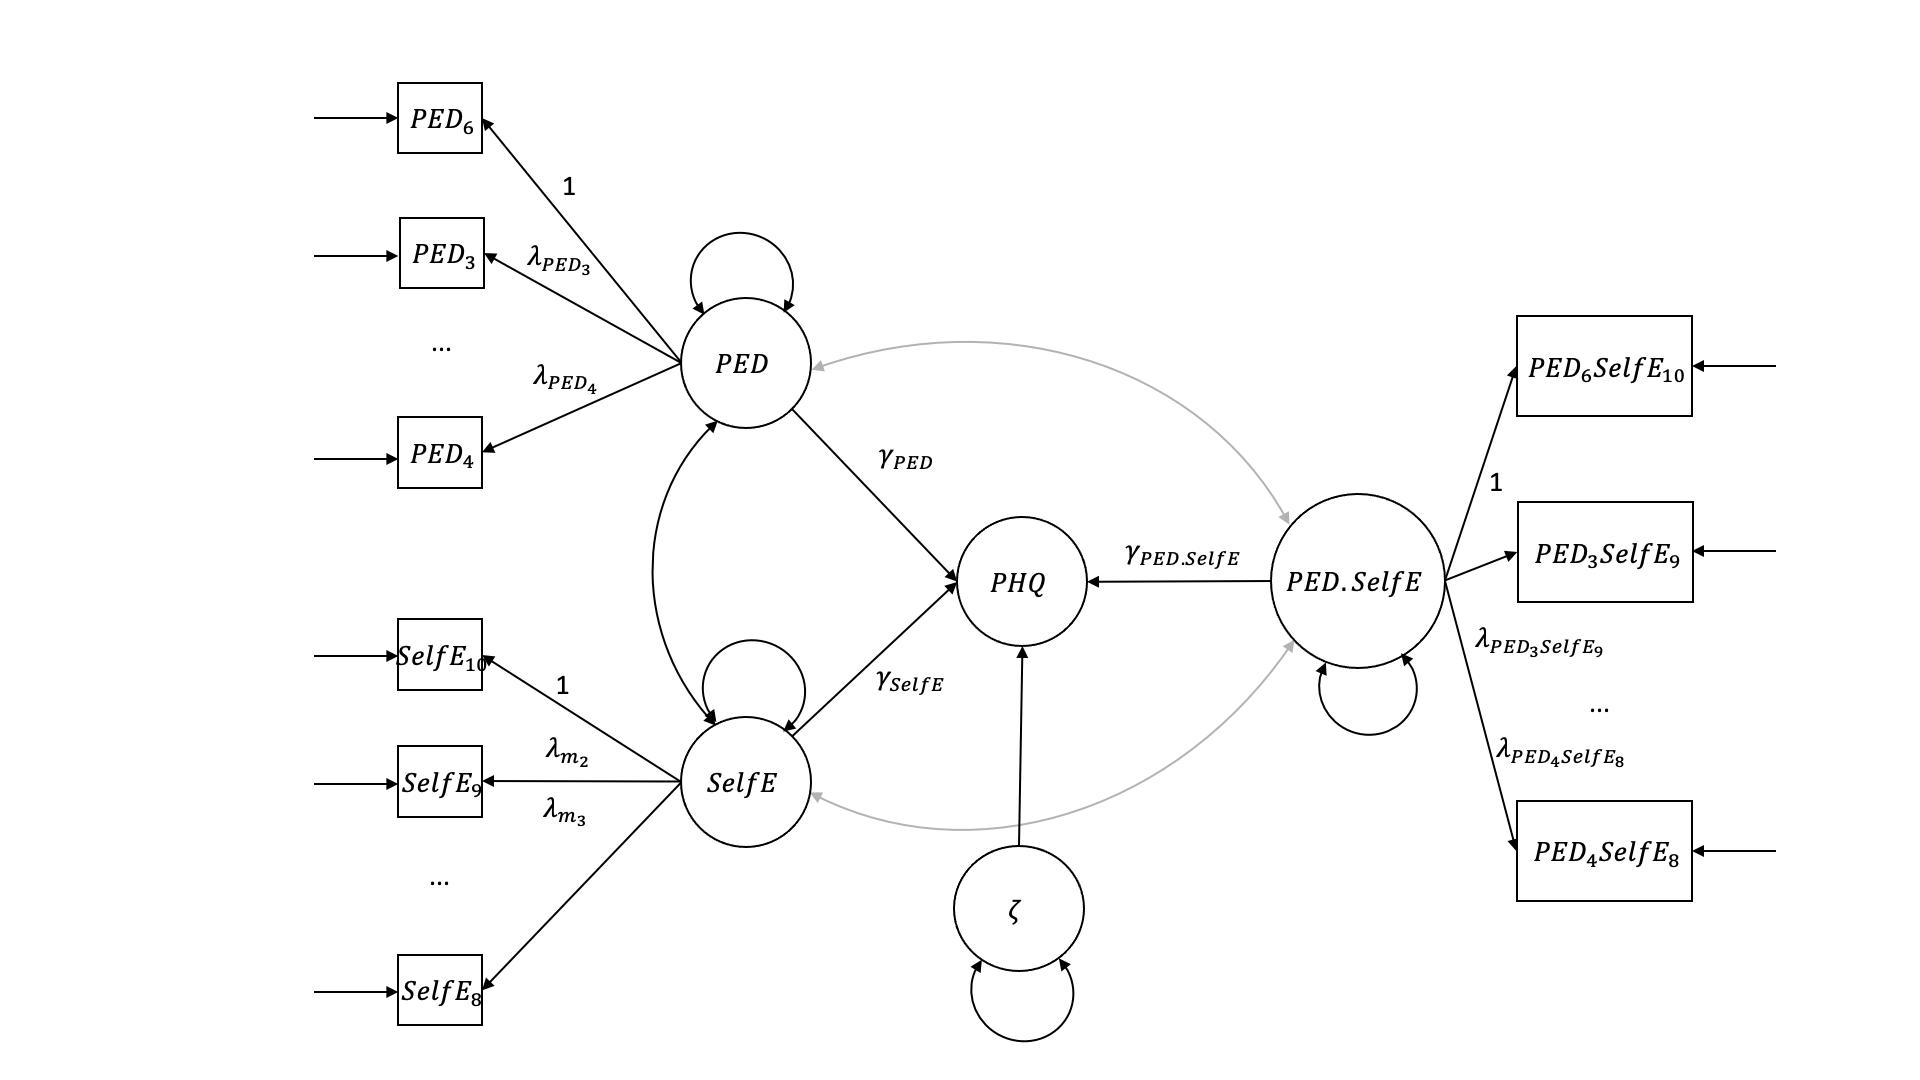
\includegraphics[width=1\linewidth]{Plots/Slide1} 

}

\caption{Hypothesized Model of Matched-Pair UPI. PED, SelfE, and PHQ represent the latent variables of perceived everyday discrimination, self-esteem, and depression, which are indicated by their corresponding first-order indicators. The latent interaction term, PED.SelfE, is indicated by formed PIs. $\zeta$ is the disturbance of PHQ. The error terms of indicators were not shown due to limited space. PED, SelfE, and PED.SelfE are allowed to correlate with each other.}\label{fig:figure-1}
\end{figure}

\begin{figure}

{\centering 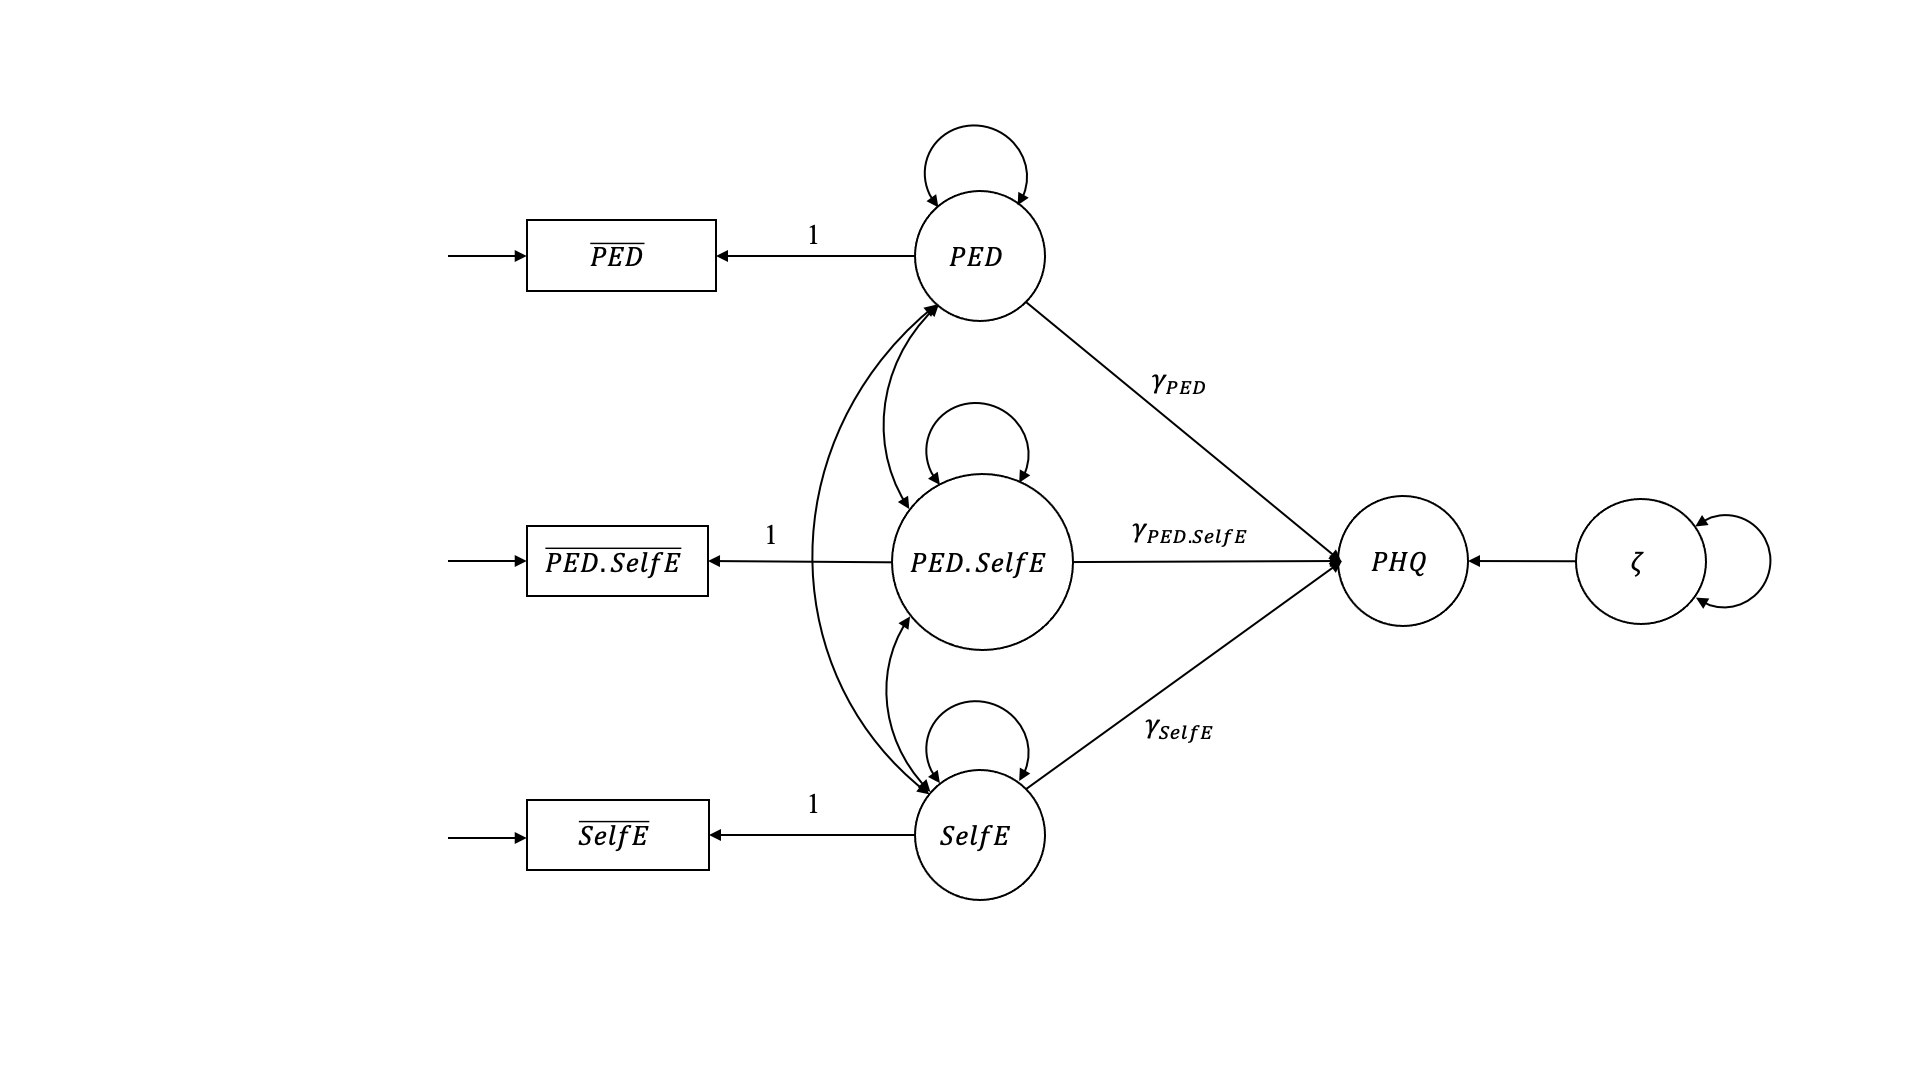
\includegraphics[width=1\linewidth]{Plots/Slide2} 

}

\caption{Hypothesized Model of RAPI. PED, SelfE, and PHQ represent the latent variables of perceived everyday discrimination, self-esteem, and depression, which are indicated by corresponding single indicators using mean scores. The latent interaction term is indicated by the product of SIs of PED and SelfE. $\zeta$ is the disturbance of PHQ. The error terms of SIs were not shown due to limited space. PED, SelfE, and PED.SelfE are allowed to correlate with each other.}\label{fig:figure-2}
\end{figure}

\begin{figure}

{\centering 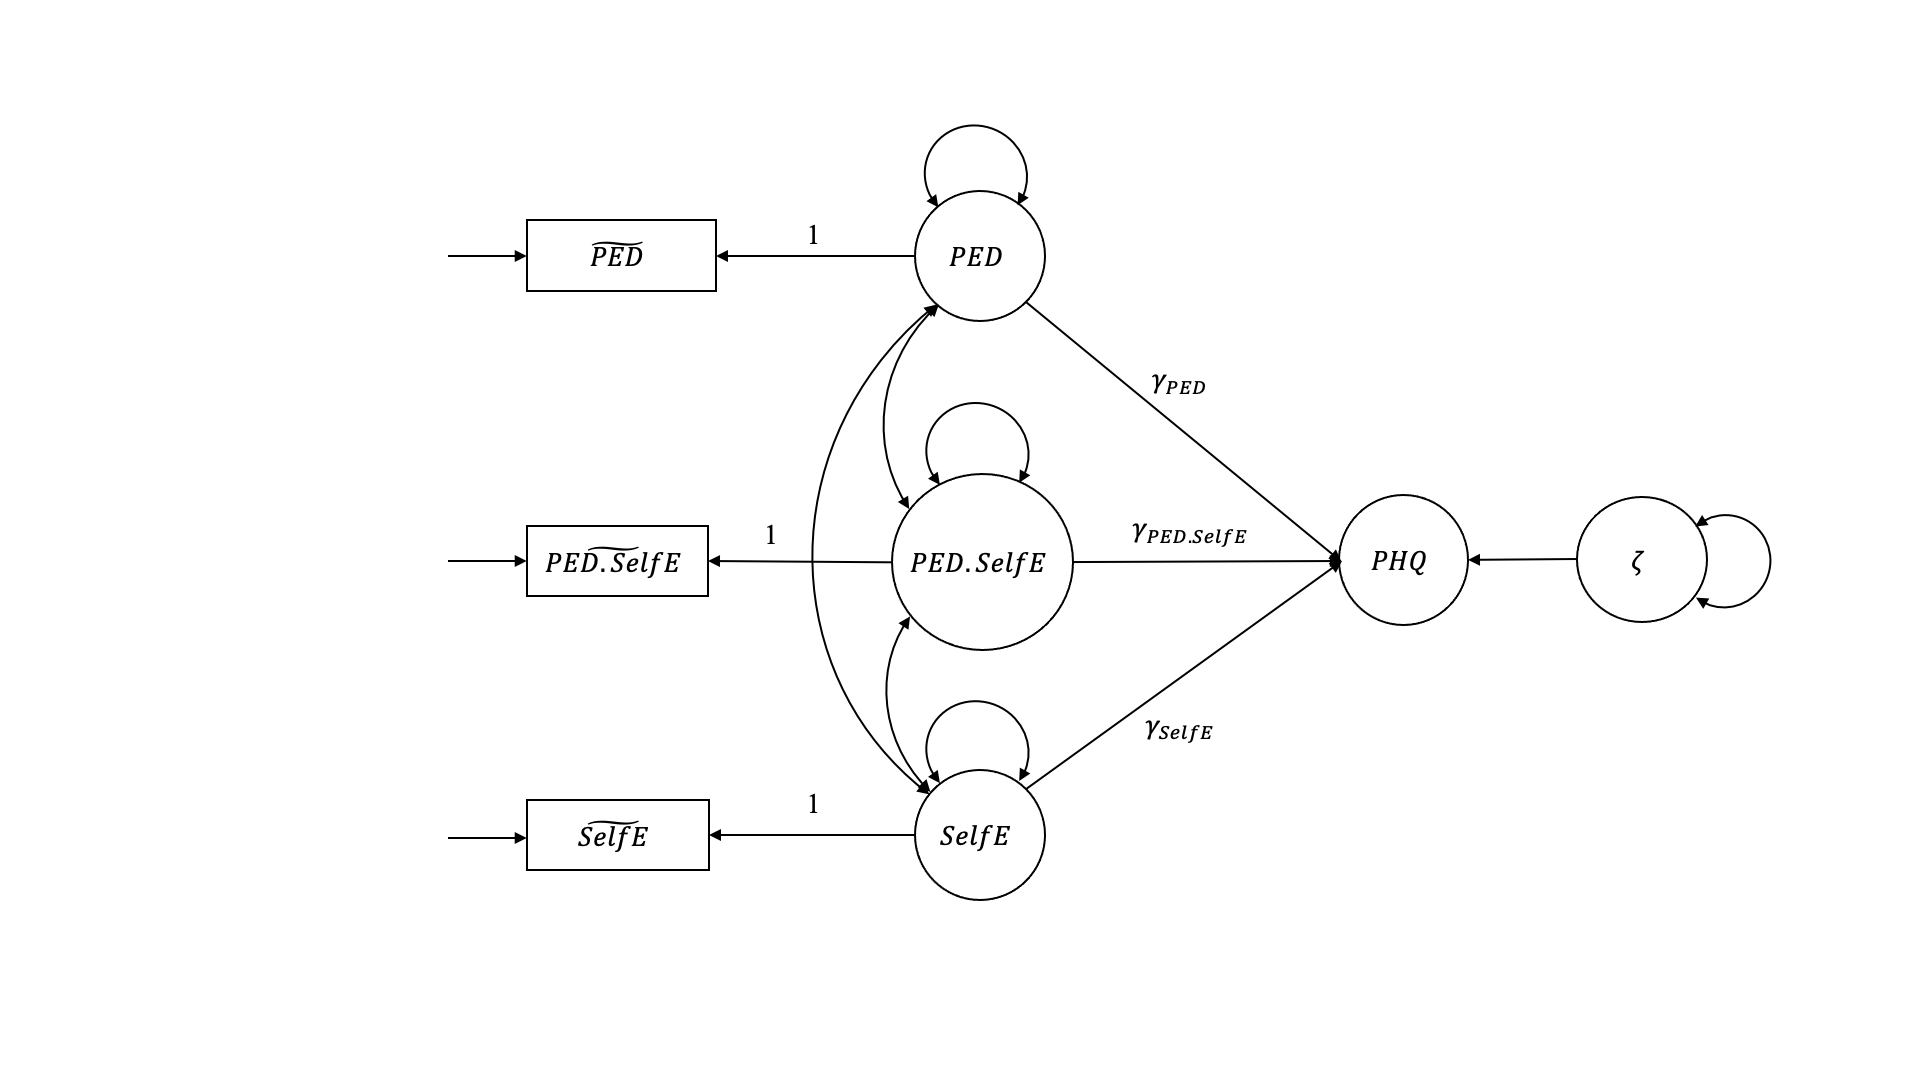
\includegraphics[width=1\linewidth]{Plots/Slide3} 

}

\caption{Hypothesized Model of 2S-PA-Int. PED, SelfE, and PHQ represent the latent variables of perceived everyday discrimination, self-esteem, and depression, which are indicated by corresponding single indicators using factor scores. The latent interaction term is indicated by the product of SIs of PED and SelfE. $\zeta$ is the disturbance of PHQ. The error terms of SIs were not shown due to limited space. PED, SelfE, and PED.SelfE are allowed to correlate with each other.}\label{fig:figure-3}
\end{figure}


\end{document}
